% The chain factor graph of Section~\ref{sec:hmm}, drawn by hand. Input by
% textbook.tex; a sketch and not a rendered figure, so it is outside the
% figure cache and the render cap, which govern generated output only.
\begin{figure}[htbp]
\centering
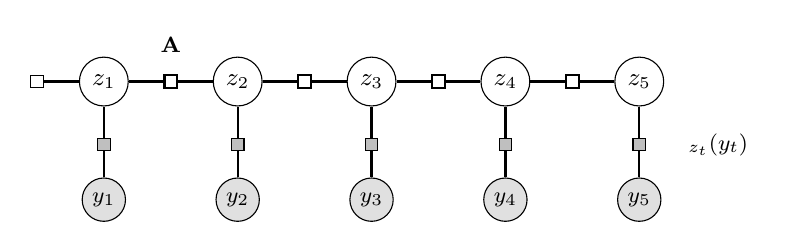
\begin{tikzpicture}[
    scale=1.0,
    state/.style={circle, draw, minimum size=0.62cm, inner sep=0.5pt, font=\small, fill=white},
    observed/.style={circle, draw, fill=black!12, minimum size=0.55cm, inner sep=0.5pt, font=\footnotesize},
    factor/.style={rectangle, draw, fill=white, minimum size=0.16cm, inner sep=0pt},
    emit/.style={rectangle, draw, fill=black!25, minimum size=0.16cm, inner sep=0pt},
    link/.style={draw, thick}
]
  \foreach \t in {1,...,5} {
    \node[state] (z\t) at (1.7*\t, 1.6) {$z_{\t}$};
    \node[emit] (e\t) at (1.7*\t, 0.8) {};
    \node[observed] (y\t) at (1.7*\t, 0.1) {$y_{\t}$};
    \draw[link] (z\t) -- (e\t) -- (y\t);
  }
  \foreach \t/\next in {1/2, 2/3, 3/4, 4/5} {
    \draw[link] (z\t) -- node[factor, pos=0.5] {} (z\next);
  }
  \node[factor] (init) at (0.85, 1.6) {};
  \draw[link] (init) -- (z1);
  \node[anchor=south, font=\footnotesize] at (0.85, 1.85) {$\bpi$};
  \node[anchor=south, font=\footnotesize] at (2.55, 1.85) {$\mathbf{A}$};
  \node[anchor=west, font=\footnotesize] at (9.0, 0.8) {$\emission_{z_t}(y_t)$};
\end{tikzpicture}
\caption{A hidden Markov model as a factor graph. Open circles are the hidden
states $z_t$ over $k$ values, open squares the transition factors
$\mathbf{A}$, the leftmost square the initial distribution $\bpi$, and shaded
squares the emission factors of the family $\emission$, each folding in one
observation $y_t$ (shaded circle). The chain is a tree, so
Equation~\ref{eq:sum-product} is exact and its two passes are
Equation~\ref{eq:forward} and Equation~\ref{eq:posterior}. Removing the
transition factors leaves the Gaussian mixture of
Section~\ref{sec:mixture}; keeping them and gating the emissions on a spatial
label gives the coupled model of Section~\ref{sec:coupled}. A sketch of the
structure and not a rendering of any instance.}
\label{fig:hmm:sketch}
\end{figure}
